\documentclass[12pt]{article}

% TEMPLATE DEFAULT PACKAGES
\usepackage{amssymb,amsmath,amsfonts,eurosym,geometry,ulem,graphicx,color,setspace,sectsty,comment,natbib,pdflscape,array,adjustbox}

% ADDED PACKAGES FOR THIS MANUSCRIPT
\usepackage{palatino,newtxmath,multirow,titlesec,threeparttable,tabu,booktabs,titlesec,threeparttable,mathtools,bm,bbm,subcaption,pdflscape,tcolorbox,mathrsfs}
% endfloat,

\usepackage{afterpage}
\usepackage[hyphens]{url}
\usepackage[margin=1cm]{caption}

\usepackage[draft]{hyperref}
\newcommand{\tim}{$\,\times\,$}
% FIGURES & TABLES CAPTION STYLING
\captionsetup[figure]{labelfont={bf},name={Figure},labelsep=period}
\captionsetup[table]{labelfont={bf},name={Table},labelsep=period}

% SECTION TITLE SETTINGS
\titlelabel{\thetitle.\enskip}
\titleformat*{\section}{\large\bfseries}
\titleformat*{\subsection}{\normalsize\bfseries}

% COLUMN TYPES
\newcolumntype{L}[1]{>{\raggedright\let\newline\\\arraybackslash\hspace{0pt}}m{#1}}
\newcolumntype{C}{>{\centering\arraybackslash}p{5.2em}}
\newcolumntype{D}{>{\centering\arraybackslash}p{5em}}
\newcolumntype{R}[1]{>{\raggedleft\let\newline\\\arraybackslash\hspace{0pt}}m{#1}}


% MARGINS AND SPACING
\normalem
\geometry{left=1.1in,right=1.1in,top=1.0in,bottom=1.0in}
\setlength{\parskip}{2.5pt}

% SPECIAL CELL 
\newcommand{\specialcell}[2][c]{%
	\begin{tabular}[#1]{@{}l@{}}#2\end{tabular}}

% NO INDENT ON FOOTNOTES
\usepackage[hang,flushmargin]{footmisc}

\begin{document}



% \vspace{0mm}
% \begin{table}[h!]
% \centering
% \caption{Housing Project Areas Description}\label{table:projectdescriptives}
% \vspace{0mm}
% \begin{tabular}{l*{1}{cccccc}}
% \toprule
%   & \multicolumn{2}{c}{\textbf{All}}& \multicolumn{2}{c}{\textbf{Greenfield}}  & \multicolumn{2}{c}{\textbf{In-Situ}}   \\
%   &Const. & Unconst. &Const. & Unconst.   & Const. & Unconst. \\
% \midrule
%  Number of Projects  & 172  & 145  & 43  & 20  & 27  & 29  \\ 
 Area (km2)  & 1.17  & 1.16  & 1.72  & 2.42  & 1.50  & 0.88  \\ 
 Median Construction Yr.  & 2006  & 2006  & 2006  & 2005  & 2004  & 2006  \\ 
 Delivered Houses  & 374  & 11  & 568  & 24  & 702  & 20  \\ 
 House Price in 1 km (R$^\dagger$)  & 188,441  & 218,635  & 194,214  & 186,841  & 179,596  & 208,570  \\ 
 Distance to CBD$^\ddagger$ (km)  & 32.5  & 27.7  & 40.5  & 39.9  & 32.6  & 30.6  \\ 

% \bottomrule
% \multicolumn{7}{l}{\scriptsize Const. refers to constructed projects and unconst. refers to unconstructed projects.}\\[-.5em]
% \multicolumn{7}{l}{\scriptsize $^*$Calculated from {\it expected} completion dates using Gauteng National Treasury budget reports.}\\[-.5em]
% \multicolumn{7}{l}{\scriptsize $^\dagger$ The USD averaged to about 7.70 Rands during the 2001-2011 period.}\\[-.5em]
% \multicolumn{7}{l}{\scriptsize $^\ddagger$Measured as the average minimum distance with respect to Johannesburg and Pretoria CBDs. } \\[-.5em]
% %\multicolumn{7}{l}{\scriptsize City includes projects whose centroids are within 30.4 km of their nearest CBD.} \\[-.5em]
% %\multicolumn{7}{l}{\scriptsize Suburb includes projects whose centroids are further than 30.4 km from their nearest CBD.}
% \end{tabular}
% \end{table} 



% \begin{figure*}
%         \centering
%    %     \caption[ Pre-Period Housing Densities in Constructed and Unconstructed Projects Areas ]
%   %      {\small Pre-Period Densities} 
%         %\vspace{2mm}
%         \begin{subfigure}[b]{0.48\textwidth}
%                     \caption[Network2]%
%             {{\footnotesize \textbf{All Projects} pre-period formal raw data}}    
%             \label{fig:prefor}
%             \centering
%             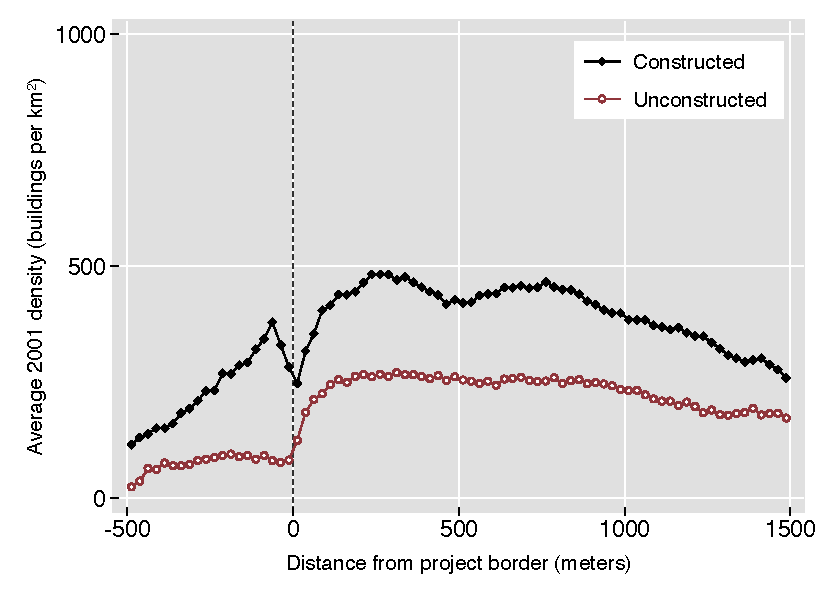
\includegraphics[width=\textwidth,trim={0.3cm .3cm 0.1cm 0cm}, clip=true]{figures/bblu_for_pre_means_4_spk.pdf}

%         \end{subfigure}
%         \hfill
%         \begin{subfigure}[b]{0.48\textwidth}  
%                     \caption[]%
%             {{\footnotesize \textbf{All Projects} pre-period informal  raw data}}      
%             \label{fig:preinf}
%             \centering 
%             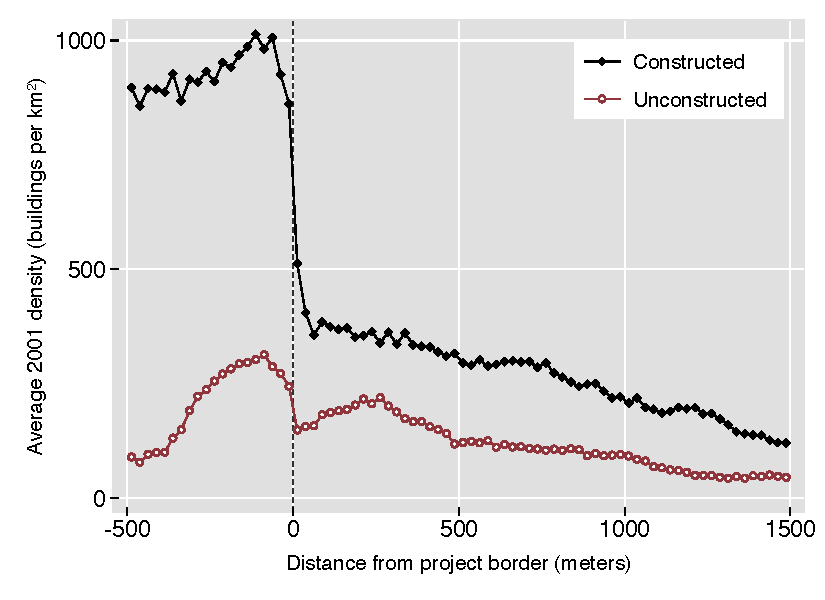
\includegraphics[width=\textwidth,trim={0.3cm .3cm 0.1cm 0cm}, clip=true]{figures/bblu_inf_pre_means_4_spk.pdf}

%         \end{subfigure}
%         \begin{subfigure}[b]{0.48\textwidth}
%                     \caption[Network2]%
%             {{\footnotesize \textbf{Greenfield} pre-period formal  raw data}}    
%             \label{fig:prefor}
%             \centering
%             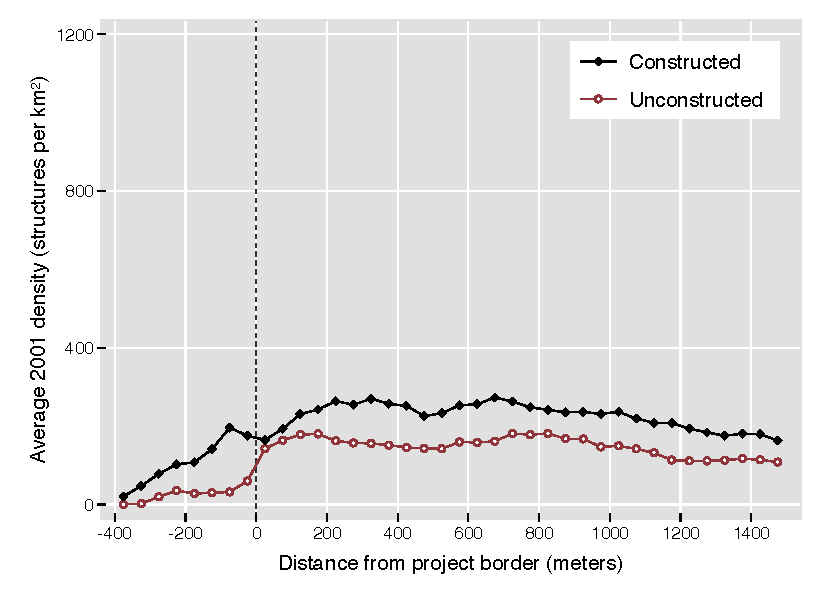
\includegraphics[width=\textwidth,trim={0.3cm .3cm 0.1cm 0cm}, clip=true]{figures/bblu_for_pre_means_4_1_spk.pdf}

%         \end{subfigure}
%         \hfill
%         \begin{subfigure}[b]{0.48\textwidth}  
%                     \caption[]%
%             {{\footnotesize \textbf{Greenfield} pre-period informal  raw data}}     
%             \label{fig:preinf}
%             \centering 
%             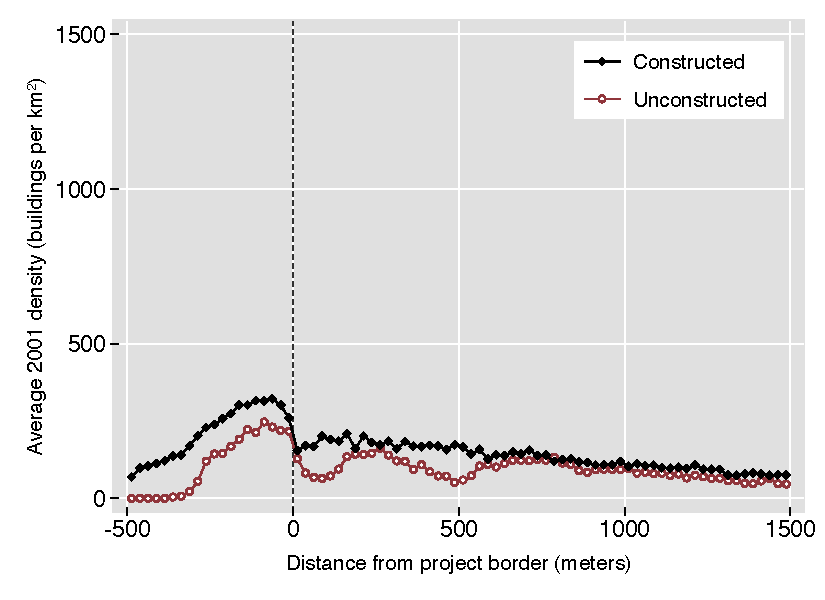
\includegraphics[width=\textwidth,trim={0.3cm .3cm 0.1cm 0cm}, clip=true]{figures/bblu_inf_pre_means_4_1_spk.pdf}

%         \end{subfigure}
%         \begin{subfigure}[b]{0.48\textwidth}
%                     \caption[Network2]%
%             {{\footnotesize \textbf{In-Situ} pre-period formal  raw data}}   
%             \label{fig:prefor}
%             \centering
%             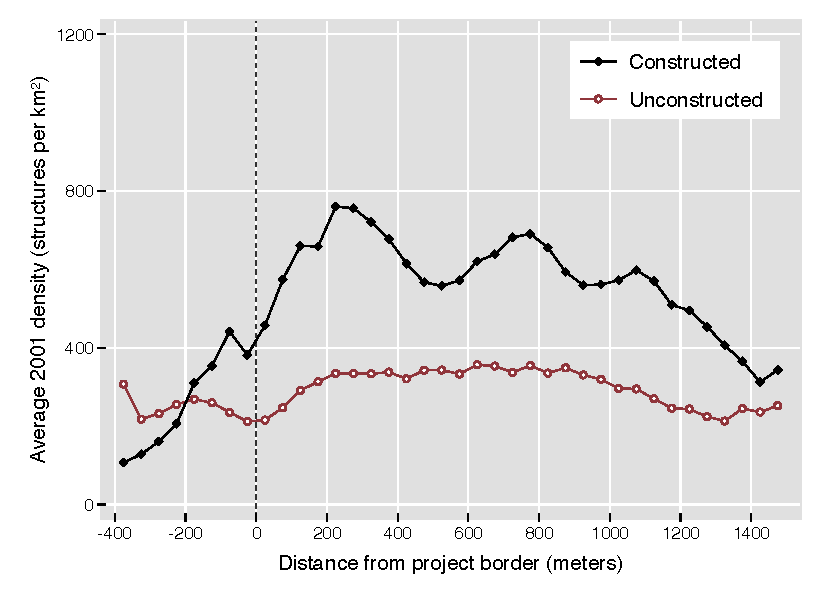
\includegraphics[width=\textwidth,trim={0.3cm .3cm 0.1cm 0cm}, clip=true]{figures/bblu_for_pre_means_4_2_spk.pdf}

%         \end{subfigure}
%         \hfill
%         \begin{subfigure}[b]{0.48\textwidth}  
%                     \caption[]%
%             {{\footnotesize \textbf{In-Situ} pre-period informal  raw data}}     
%             \label{fig:preinf}
%             \centering 
%             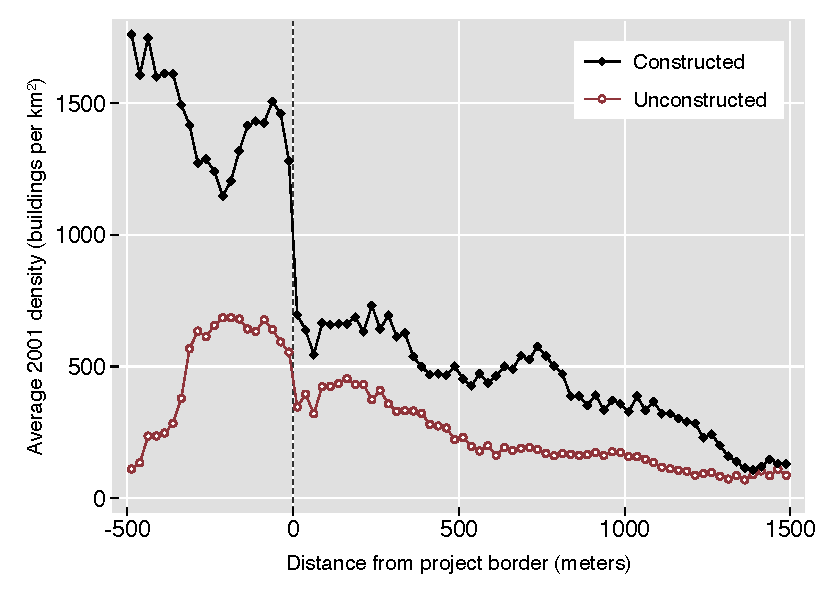
\includegraphics[width=\textwidth,trim={0.3cm .3cm 0.1cm 0cm}, clip=true]{figures/bblu_inf_pre_means_4_2_spk.pdf}

%         \end{subfigure}
%         \begin{subfigure}[b]{0.48\textwidth}
%                     \caption[Network2]%
%             {{\footnotesize \textbf{Other} pre-period formal  raw data}}   
%             \label{fig:prefor}
%             \centering
%             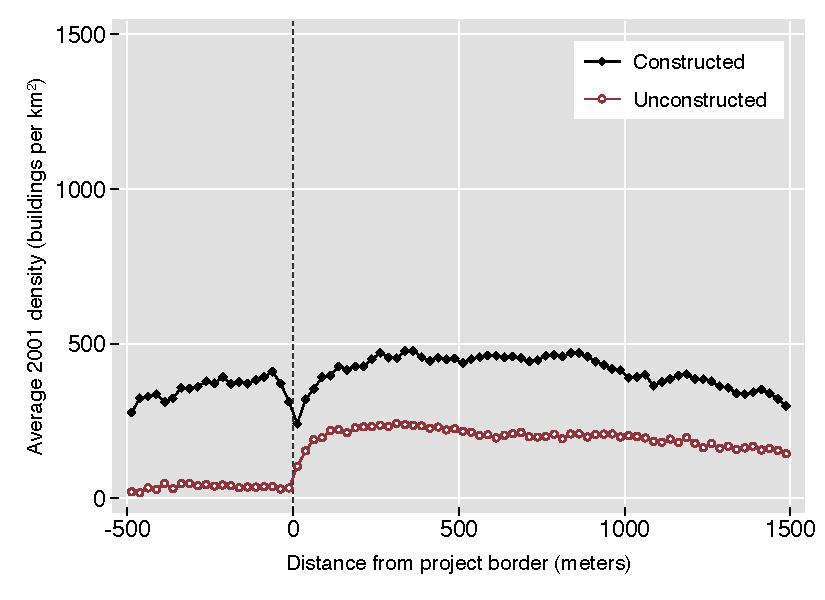
\includegraphics[width=\textwidth,trim={0.3cm .3cm 0.1cm 0cm}, clip=true]{figures/bblu_for_pre_means_4_3_spk.pdf}

%         \end{subfigure}
%         \hfill
%         \begin{subfigure}[b]{0.48\textwidth}  
%                     \caption[]%
%             {{\footnotesize \textbf{Other} pre-period informal  raw data}}      
%             \label{fig:preinf}
%             \centering 
%             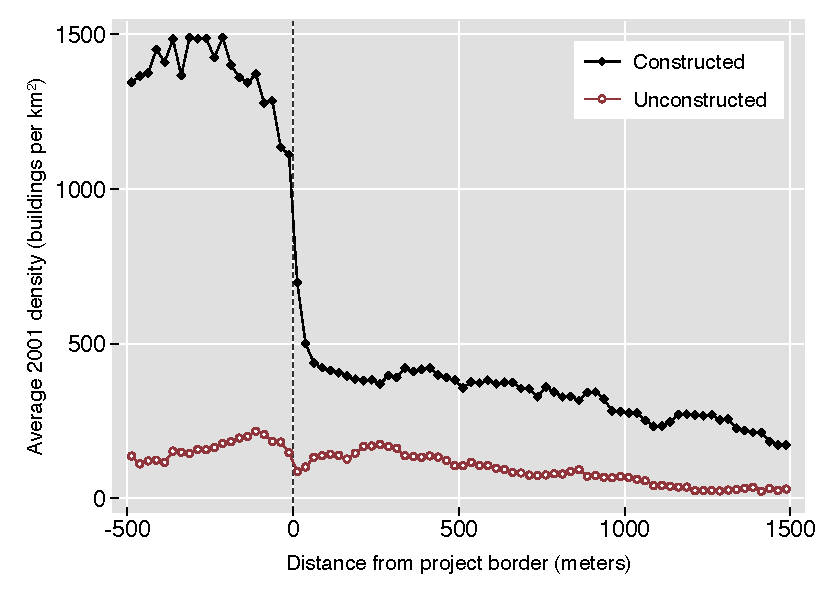
\includegraphics[width=\textwidth,trim={0.3cm .3cm 0.1cm 0cm}, clip=true]{figures/bblu_inf_pre_means_4_3_spk.pdf}

%         \end{subfigure}
% \end{figure*}








% \begin{figure*}
%         \centering
%    %     \caption[ Pre-Period Housing Densities in Constructed and Unconstructed Projects Areas ]
%   %      {\small Pre-Period Densities} 
%         %\vspace{2mm}
%         \begin{subfigure}[b]{0.48\textwidth}
%             \caption[Network2]%
%             {{\footnotesize \textbf{All Projects} changes formal raw data}}    
%             \label{fig:prefor}
%             \centering
%             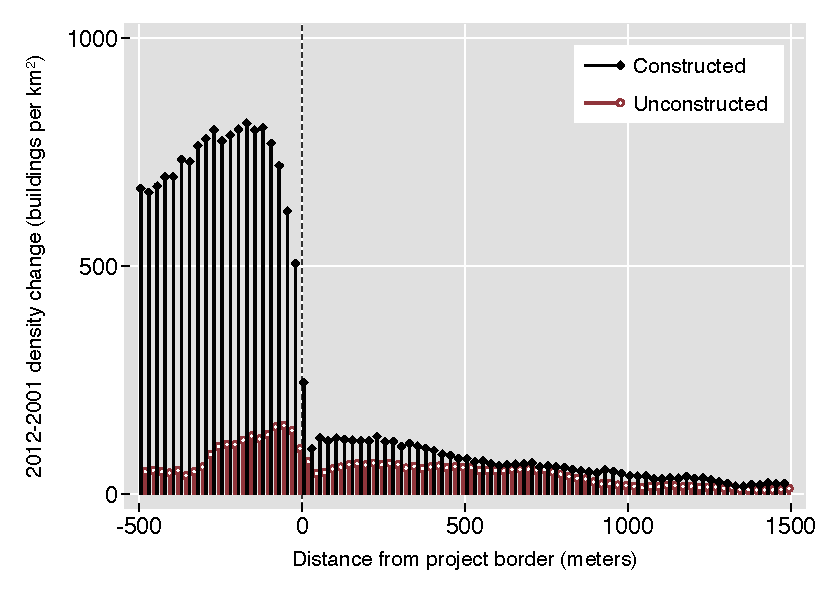
\includegraphics[width=\textwidth,trim={0.3cm .3cm 0.1cm 0cm}, clip=true]{figures/bblu_for_rawchanges_4_spk.pdf}

%         \end{subfigure}
%         \hfill
%         \begin{subfigure}[b]{0.48\textwidth}  
%                     \caption[]%
%             {{\footnotesize \textbf{All Projects} changes informal  raw data}}      
%             \label{fig:preinf}
%             \centering 
%             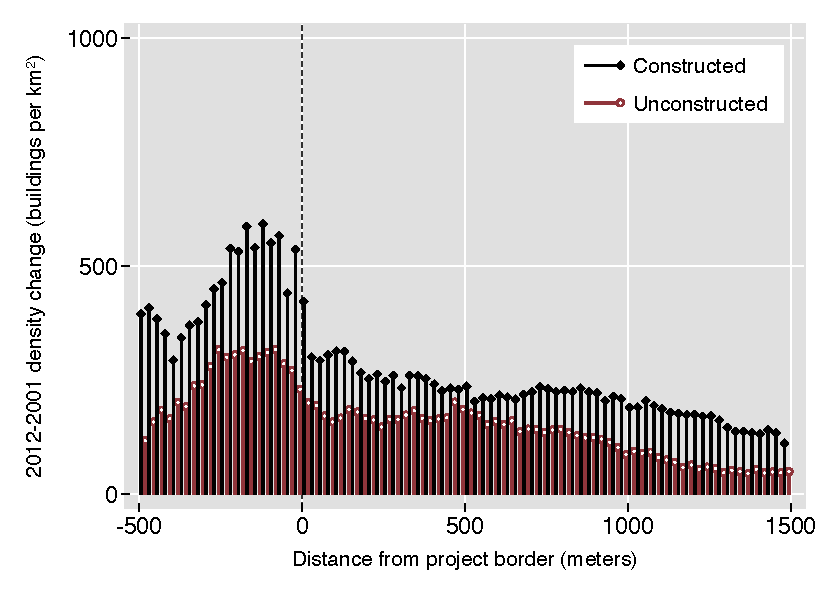
\includegraphics[width=\textwidth,trim={0.3cm .3cm 0.1cm 0cm}, clip=true]{figures/bblu_inf_rawchanges_4_spk.pdf}

%         \end{subfigure}
%         \begin{subfigure}[b]{0.48\textwidth}
%                     \caption[Network2]%
%             {{\footnotesize \textbf{Greenfield} changes formal  raw data}}    
%             \label{fig:prefor}
%             \centering
%             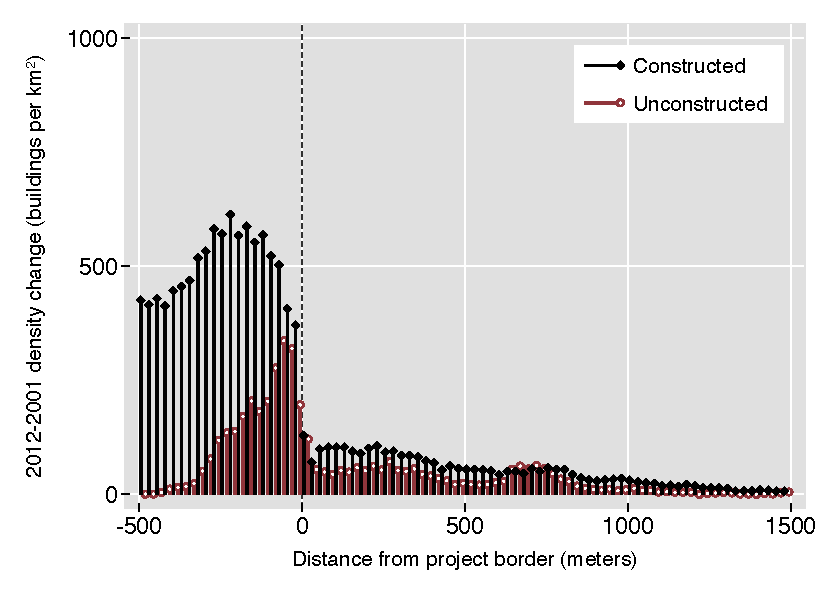
\includegraphics[width=\textwidth,trim={0.3cm .3cm 0.1cm 0cm}, clip=true]{figures/bblu_for_rawchanges_4_1_spk.pdf}

%         \end{subfigure}
%         \hfill
%         \begin{subfigure}[b]{0.48\textwidth}  
%                     \caption[]%
%             {{\footnotesize \textbf{Greenfield} changes informal raw data }}     
%             \label{fig:preinf}
%             \centering 
%             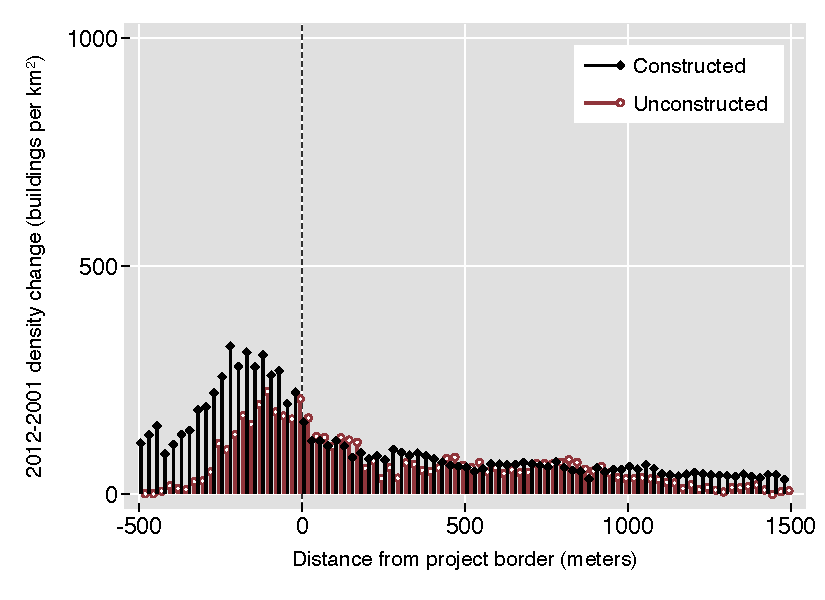
\includegraphics[width=\textwidth,trim={0.3cm .3cm 0.1cm 0cm}, clip=true]{figures/bblu_inf_rawchanges_4_1_spk.pdf}

%         \end{subfigure}
%         \begin{subfigure}[b]{0.48\textwidth}
%                     \caption[Network2]%
%             {{\footnotesize \textbf{In-Situ} changes formal raw data }}   
%             \label{fig:prefor}
%             \centering
%             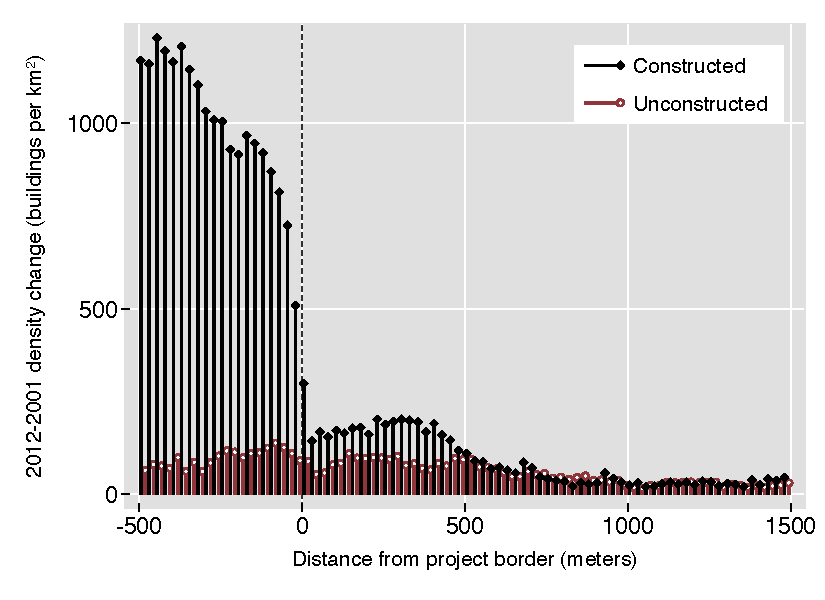
\includegraphics[width=\textwidth,trim={0.3cm .3cm 0.1cm 0cm}, clip=true]{figures/bblu_for_rawchanges_4_2_spk.pdf}

%         \end{subfigure}
%         \hfill
%         \begin{subfigure}[b]{0.48\textwidth}  
%                     \caption[]%
%             {{\footnotesize \textbf{In-Situ} changes informal raw data }}     
%             \label{fig:preinf}
%             \centering 
%             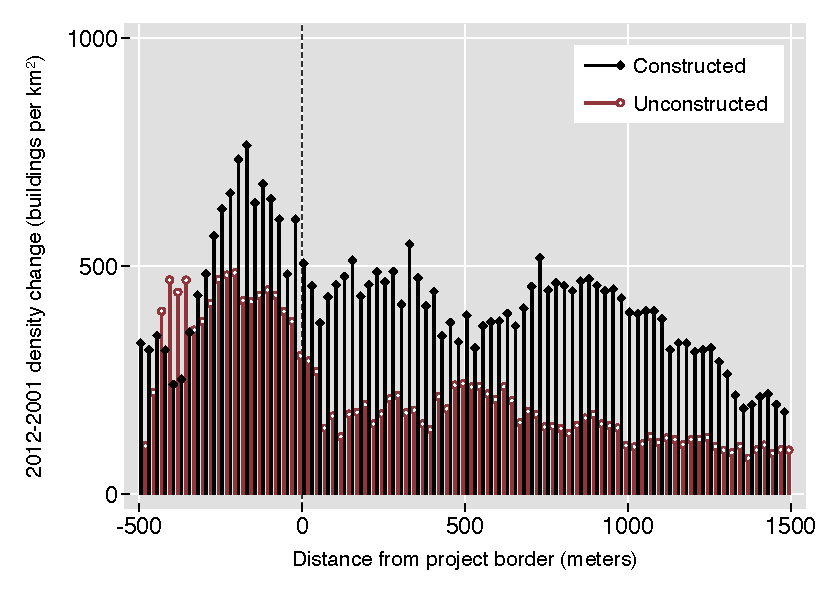
\includegraphics[width=\textwidth,trim={0.3cm .3cm 0.1cm 0cm}, clip=true]{figures/bblu_inf_rawchanges_4_2_spk.pdf}

%         \end{subfigure}
%         \begin{subfigure}[b]{0.48\textwidth}
%                     \caption[Network2]%
%             {{\footnotesize \textbf{Other} changes formal raw data}}   
%             \label{fig:prefor}
%             \centering
%             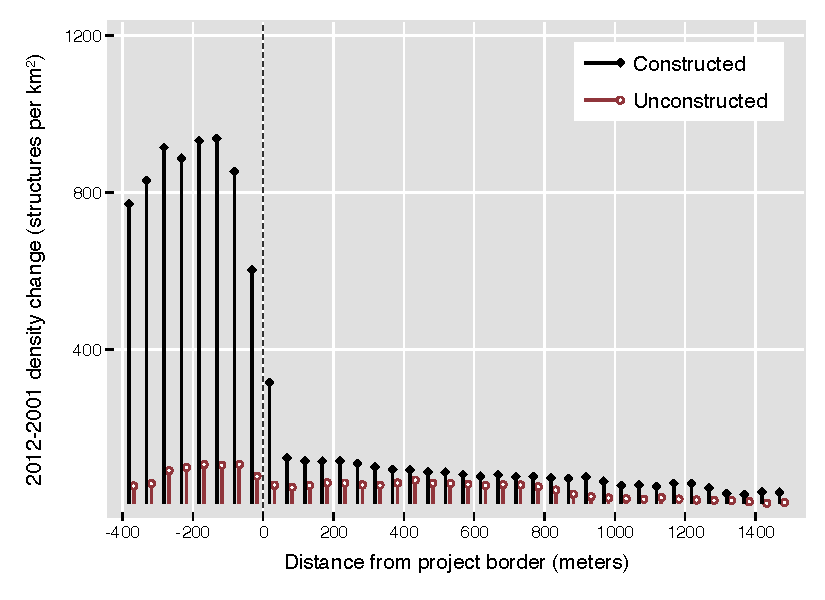
\includegraphics[width=\textwidth,trim={0.3cm .3cm 0.1cm 0cm}, clip=true]{figures/bblu_for_rawchanges_4_3_spk.pdf}

%         \end{subfigure}
%         \hfill
%         \begin{subfigure}[b]{0.48\textwidth} 
%                     \caption[]%
%             {{\footnotesize \textbf{Other} changes informal  raw data}}      
%             \label{fig:preinf} 
%             \centering 
%             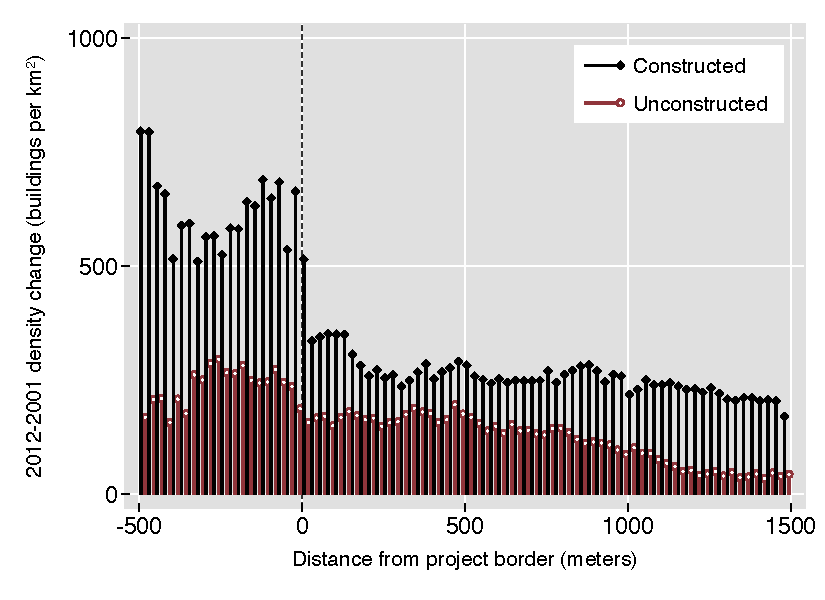
\includegraphics[width=\textwidth,trim={0.3cm .3cm 0.1cm 0cm}, clip=true]{figures/bblu_inf_rawchanges_4_3_spk.pdf}

%         \end{subfigure}
% \end{figure*}







\begin{table}
\caption{Building Density}
\begin{tabular}{lDDDDD}
\toprule
 & \small (1) & \small (2)  & \small (3) & \small (4) & \small (5) \\
 & Total & Formal  & Informal & Informal Bkyd. & Informal Non-Bkyd. \\ \midrule
\textbf{All Projects} \\inside project      &     796.780\textsuperscript{a}&     615.333\textsuperscript{a}&     181.446\textsuperscript{c}&     566.119\textsuperscript{a}&    -384.673\textsuperscript{a}\\
                    &   (147.465)                   &    (75.095)                   &   (102.220)                   &   (106.935)                   &    (82.183)                   \\[0.5em]
0-250m outside project &      94.919                   &      57.302\textsuperscript{b}&      37.617                   &      69.596                   &     -31.979                   \\
                    &    (65.290)                   &    (27.335)                   &    (54.941)                   &    (48.590)                   &    (34.114)                   \\[0.5em]
R$^2$               &       0.070                   &       0.049                   &       0.060                   &       0.048                   &       0.045                   \\

\midrule
\textbf{Greenfield} \\   inside project      &     454.687\textsuperscript{b}&     337.175\textsuperscript{b}&     117.512                   &     203.699\textsuperscript{c}&     -86.187                   \\
                    &   (220.370)                   &   (146.212)                   &    (96.048)                   &   (108.255)                   &    (64.278)                   \\[0.01em]
0-250m outside project &     -76.487                   &     -44.537                   &     -31.950                   &     -24.936                   &      -7.014                   \\
                    &   (120.739)                   &    (63.090)                   &    (69.564)                   &    (56.512)                   &    (46.647)                   \\[0.8em] 
\textbf{In-Situ Upgrading} \\   inside project      &     909.829\textsuperscript{b}&     912.548\textsuperscript{a}&      -2.719                   &     821.193\textsuperscript{a}&    -823.913\textsuperscript{a}\\
                    &   (398.411)                   &   (164.030)                   &   (315.764)                   &   (283.114)                   &   (229.096)                   \\[0.01em]
0-250m outside project &     297.323                   &     175.919                   &     121.404                   &     179.322                   &     -57.918                   \\
                    &   (233.684)                   &   (114.045)                   &   (186.861)                   &   (167.334)                   &   (120.645)                   \\[0.8em]
\textbf{Other} \\   inside project      &     955.298\textsuperscript{a}&     685.454\textsuperscript{a}&     269.844\textsuperscript{c}&     694.935\textsuperscript{a}&    -425.091\textsuperscript{a}\\
                    &   (183.984)                   &    (81.155)                   &   (146.116)                   &   (125.878)                   &   (102.162)                   \\[0.01em]
0-250m outside project &      82.699                   &      59.129                   &      23.570                   &      52.840                   &     -29.270                   \\
                    &   (104.634)                   &    (43.100)                   &    (83.729)                   &    (69.371)                   &    (47.766)                   \\[0.8em]
Mean Outcome 2001   &      526.22                   &      261.56                   &      264.66                   &       96.43                   &      168.23                   \\
Mean Outcome 2011   &      838.62                   &      385.14                   &      453.48                   &      286.79                   &      166.69                   \\
R$^2$               &       0.113                   &       0.069                   &       0.101                   &       0.076                   &       0.073                   \\
N                   &   1,705,534                   &   1,705,534                   &   1,705,534                   &   1,705,534                   &   1,705,534                   \\

\bottomrule
\end{tabular}
\end{table}





\begin{table}[h!] 
\caption{Effect of Housing Projects on Socio-demographics}
\label{table:sorting}
\small
\centering
%\caption{Census Composition Estimates }
\vspace{-2mm}
\begin{tabular}{lDDDDD}
\toprule
& \small (1) & \small (2) & \small (3) & \small (4)& \small (5)\\
& \small Age & \small P.O.B. not Gauteng & \small Unemployed & \small Years of Education & \small Monthly Income \\ \midrule 
\textbf{All Projects} \\inside project      &       0.200                   &      -0.044                   &       0.012                   &       0.282\textsuperscript{c}&    1758.695\textsuperscript{a}\\
                    &     (0.328)                   &     (0.030)                   &     (0.020)                   &     (0.154)                   &   (508.517)                   \\[0.5em]
0-250m outside project &       0.281                   &       0.011                   &       0.007                   &       0.132                   &     812.774                   \\
                    &     (0.347)                   &     (0.028)                   &     (0.022)                   &     (0.133)                   &   (569.076)                   \\[0.5em]
R$^2$               &       0.179                   &       0.105                   &       0.196                   &       0.374                   &       0.171                   \\

\midrule
\textbf{Greenfield} \\   inside project      &      -2.003\textsuperscript{a}&      -0.006                   &       0.063                   &      -0.707                   &     494.949                   \\
                    &     (0.714)                   &     (0.067)                   &     (0.053)                   &     (0.453)                   &  (1201.071)                   \\[0.01em]
0-250m outside project &      -1.400\textsuperscript{b}&      -0.047                   &       0.059                   &      -0.697\textsuperscript{b}&    -932.249                   \\
                    &     (0.670)                   &     (0.052)                   &     (0.051)                   &     (0.327)                   &   (889.309)                   \\[0.8em] 
\textbf{In-Situ Upgrading} \\   inside project      &       0.560                   &      -0.130\textsuperscript{b}&       0.029                   &       0.222                   &    1405.305                   \\
                    &     (0.815)                   &     (0.062)                   &     (0.033)                   &     (0.253)                   &  (1179.104)                   \\[0.01em]
0-250m outside project &      -0.137                   &      -0.040                   &       0.047                   &       0.205                   &    1194.176                   \\
                    &     (0.808)                   &     (0.064)                   &     (0.042)                   &     (0.273)                   &  (1285.601)                   \\[0.8em]
\textbf{Other} \\   inside project      &       0.524                   &       0.022                   &      -0.005                   &       0.536\textsuperscript{b}&    2388.064\textsuperscript{a}\\
                    &     (0.500)                   &     (0.043)                   &     (0.031)                   &     (0.215)                   &   (842.591)                   \\[0.01em]
0-250m outside project &       0.883                   &       0.045                   &      -0.027                   &       0.294                   &    1201.443                   \\
                    &     (0.576)                   &     (0.043)                   &     (0.031)                   &     (0.184)                   &   (941.052)                   \\[0.8em]
Mean Outcome 2001   &       27.30                   &        0.37                   &        0.47                   &        8.27                   &    2,477.01                   \\
Mean Outcome 2011   &       28.30                   &        0.43                   &        0.33                   &        9.68                   &    4,486.48                   \\
R$^2$               &       0.192                   &       0.136                   &       0.201                   &       0.389                   &       0.190                   \\
N                   &      12,734                   &      12,727                   &      12,724                   &      12,728                   &      12,724                   \\

\bottomrule
\multicolumn{6}{l}{\footnotesize Standard errors clustered at the project level in parenthesis. \textsuperscript{c} p$<$0.10, \textsuperscript{b} p$<$0.05, \textsuperscript{a} p$<$0.01  }\\
\multicolumn{6}{l}{\footnotesize P.O.B. means ``place of birth.''  Monthly income is in Rands.}
\end{tabular}
\end{table}








\begin{landscape}
{\footnotesize

\begin{table}[]
\small
\centering
\caption{Census Household-level Estimates }\label{table:censusestimates}
\vspace{-2mm}
\resizebox{.9\linewidth}{!}{
\begin{tabular}{lDDDDDDDD}
\toprule
 & \small (1) & \small (2)  & \small (3) & \small (4) & \small (5)  & \small (6)  & \small (7) & (8)\\
 & \small Flush Toilet & \small Water Indoors  & \small Electricity Cooking & \small Electricity Heating & \small Electricity Lighting  & \small Number of Rooms  & \small Household Size & Population Density\\ \midrule 
\textbf{All Projects} \\inside project      &       0.104                   &       0.193\textsuperscript{a}&       0.231\textsuperscript{a}&       0.167\textsuperscript{b}&       0.109                   &       0.297                   &       0.145                   &   -3492.994                   \\
                    &     (0.085)                   &     (0.053)                   &     (0.087)                   &     (0.081)                   &     (0.088)                   &     (0.190)                   &     (0.120)                   &  (2281.678)                   \\[0.5em]
0-250m outside project &      -0.040                   &       0.054                   &       0.008                   &      -0.002                   &      -0.009                   &       0.127                   &       0.010                   &   -1471.210                   \\
                    &     (0.053)                   &     (0.051)                   &     (0.055)                   &     (0.059)                   &     (0.048)                   &     (0.162)                   &     (0.080)                   &  (1650.946)                   \\[0.5em]
R$^2$               &       0.096                   &       0.147                   &       0.181                   &       0.163                   &       0.098                   &       0.098                   &       0.095                   &       0.012                   \\

\midrule
\textbf{Greenfield} \\   inside project      &      -0.057                   &       0.106                   &       0.037                   &      -0.012                   &       0.039                   &       0.070                   &       0.233                   &    5935.335                   \\
                    &     (0.156)                   &     (0.133)                   &     (0.120)                   &     (0.134)                   &     (0.134)                   &     (0.403)                   &     (0.157)                   &  (3686.145)                   \\[0.01em]
0-250m outside project &      -0.099                   &       0.025                   &      -0.072                   &      -0.053                   &       0.034                   &       0.131                   &       0.418\textsuperscript{a}&    6908.049                   \\
                    &     (0.086)                   &     (0.118)                   &     (0.108)                   &     (0.115)                   &     (0.063)                   &     (0.337)                   &     (0.154)                   &  (4426.127)                   \\[0.8em] 
\textbf{In-Situ Upgrading} \\   inside project      &       0.367\textsuperscript{b}&       0.167                   &       0.291\textsuperscript{c}&       0.258\textsuperscript{c}&       0.193                   &       0.829\textsuperscript{b}&       0.501\textsuperscript{b}&   -8792.939\textsuperscript{c}\\
                    &     (0.155)                   &     (0.103)                   &     (0.150)                   &     (0.142)                   &     (0.129)                   &     (0.371)                   &     (0.249)                   &  (5296.588)                   \\[0.01em]
0-250m outside project &       0.006                   &      -0.008                   &       0.042                   &       0.022                   &       0.030                   &       0.130                   &       0.174                   &   -3654.792                   \\
                    &     (0.125)                   &     (0.117)                   &     (0.129)                   &     (0.144)                   &     (0.101)                   &     (0.378)                   &     (0.174)                   &  (3514.926)                   \\[0.8em]
\textbf{Other} \\   inside project      &      -0.047                   &       0.229\textsuperscript{a}&       0.180                   &       0.108                   &       0.023                   &       0.009                   &      -0.142                   &   -3565.574                   \\
                    &     (0.108)                   &     (0.074)                   &     (0.116)                   &     (0.107)                   &     (0.126)                   &     (0.294)                   &     (0.144)                   &  (2886.847)                   \\[0.01em]
0-250m outside project &      -0.043                   &       0.099                   &       0.003                   &      -0.006                   &      -0.037                   &       0.194                   &      -0.159                   &   -2886.289                   \\
                    &     (0.065)                   &     (0.068)                   &     (0.067)                   &     (0.071)                   &     (0.061)                   &     (0.264)                   &     (0.119)                   &  (2838.252)                   \\[0.8em]
Mean Outcome 2001   &        0.79                   &        0.35                   &        0.66                   &        0.62                   &        0.77                   &        3.30                   &        3.51                   &    8,566.83                   \\
Mean Outcome 2011   &        0.83                   &        0.54                   &        0.81                   &        0.72                   &        0.82                   &        3.56                   &        3.18                   &    9,823.82                   \\
R$^2$               &       0.108                   &       0.170                   &       0.200                   &       0.184                   &       0.118                   &       0.111                   &       0.107                   &       0.046                   \\
N                   &      12,732                   &      12,732                   &      12,732                   &      12,732                   &      12,732                   &      12,709                   &      12,730                   &      12,734                   \\

\bottomrule
\multicolumn{9}{l}{\footnotesize All regressions include 3km grid Fixed-Effects. Standard errors clustered at the project level in parenthesis. \textsuperscript{c} p$<$0.10,\textsuperscript{b} p$<$0.05,\textsuperscript{a} p$<$0.01 }
\end{tabular}
}
\end{table}

}
\end{landscape}




\begin{table}
\small
\centering
\caption{Triple Difference Estimates on Log-Prices}\label{table:priceDDD_het}
\vspace{-2mm}
\begin{tabular}{lCC}
\toprule
 & \small (1) & \small (2)  \\ \midrule 
 \textbf{All Projects} \\
 inside project      &       0.361                   &       0.366                   \\
                    &     (0.543)                   &     (0.544)                   \\[0.5em]
0-250m outside project &      -0.177                   &      -0.176                   \\
                    &     (0.209)                   &     (0.209)                   \\[0.5em]
Lot Size Controls   &                               &  \checkmark                   \\
r2                  &        0.18                   &        0.18                   \\
N                   &      67,751                   &      67,751                   \\

 \midrule
\textbf{Greenfield} \\   inside project      &       0.379                   &       0.372                   \\
                    &     (0.433)                   &     (0.432)                   \\[0.01em]
0-250m outside project &      -0.290                   &      -0.295                   \\
                    &     (0.368)                   &     (0.371)                   \\[0.8em]
\textbf{In-Situ Upgrading} \\   inside project      &       0.409                   &       0.424                   \\
                    &     (0.521)                   &     (0.525)                   \\[0.01em]
0-250m outside project &      -0.133                   &      -0.131                   \\
                    &     (0.372)                   &     (0.372)                   \\[0.8em]
\textbf{Other} \\   inside project      &      -0.754                   &      -0.753                   \\
                    &     (0.549)                   &     (0.549)                   \\[0.01em]
0-250m outside project &      -0.176                   &      -0.175                   \\
                    &     (0.231)                   &     (0.231)                   \\[0.8em]
Lot Size Controls   &                               &  \checkmark                   \\
r2                  &        0.21                   &        0.21                   \\
N                   &      67,751                   &      67,751                   \\

\bottomrule
\multicolumn{3}{l}{\footnotesize Standard errors clustered at the project level in parenthesis.} \\
\multicolumn{3}{l}{ \textsuperscript{c} p$<$0.10,\textsuperscript{b} p$<$0.05,\textsuperscript{a} p$<$0.01 }
\end{tabular}
\end{table} 

% \begin{figure}
% 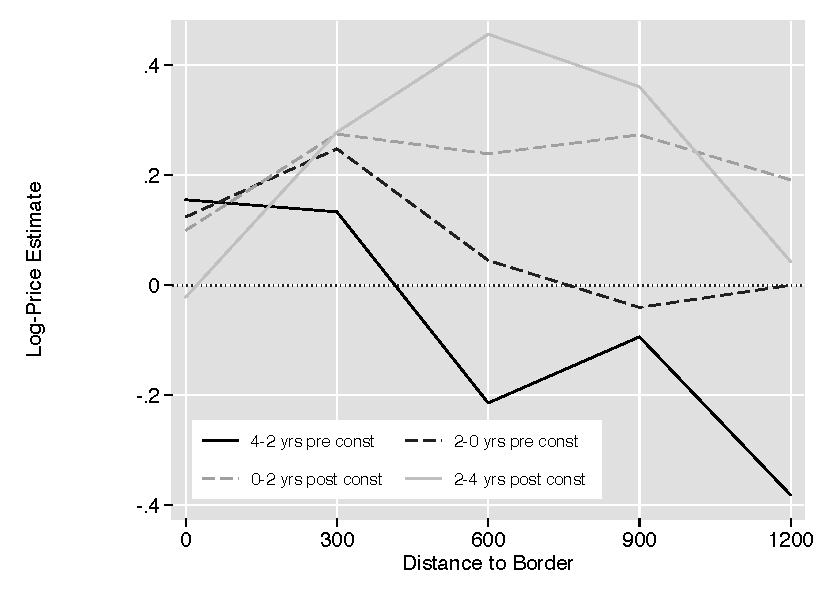
\includegraphics{figures/price_to_event_30.pdf}
% \end{figure}


\end{document}


